% Options for packages loaded elsewhere
\PassOptionsToPackage{unicode}{hyperref}
\PassOptionsToPackage{hyphens}{url}
%
\documentclass[
]{article}
\usepackage{amsmath,amssymb}
\usepackage{lmodern}
\usepackage{iftex}
\ifPDFTeX
  \usepackage[T1]{fontenc}
  \usepackage[utf8]{inputenc}
  \usepackage{textcomp} % provide euro and other symbols
\else % if luatex or xetex
  \usepackage{unicode-math}
  \defaultfontfeatures{Scale=MatchLowercase}
  \defaultfontfeatures[\rmfamily]{Ligatures=TeX,Scale=1}
\fi
% Use upquote if available, for straight quotes in verbatim environments
\IfFileExists{upquote.sty}{\usepackage{upquote}}{}
\IfFileExists{microtype.sty}{% use microtype if available
  \usepackage[]{microtype}
  \UseMicrotypeSet[protrusion]{basicmath} % disable protrusion for tt fonts
}{}
\makeatletter
\@ifundefined{KOMAClassName}{% if non-KOMA class
  \IfFileExists{parskip.sty}{%
    \usepackage{parskip}
  }{% else
    \setlength{\parindent}{0pt}
    \setlength{\parskip}{6pt plus 2pt minus 1pt}}
}{% if KOMA class
  \KOMAoptions{parskip=half}}
\makeatother
\usepackage{xcolor}
\usepackage[margin=1in]{geometry}
\usepackage{graphicx}
\makeatletter
\def\maxwidth{\ifdim\Gin@nat@width>\linewidth\linewidth\else\Gin@nat@width\fi}
\def\maxheight{\ifdim\Gin@nat@height>\textheight\textheight\else\Gin@nat@height\fi}
\makeatother
% Scale images if necessary, so that they will not overflow the page
% margins by default, and it is still possible to overwrite the defaults
% using explicit options in \includegraphics[width, height, ...]{}
\setkeys{Gin}{width=\maxwidth,height=\maxheight,keepaspectratio}
% Set default figure placement to htbp
\makeatletter
\def\fps@figure{htbp}
\makeatother
\setlength{\emergencystretch}{3em} % prevent overfull lines
\providecommand{\tightlist}{%
  \setlength{\itemsep}{0pt}\setlength{\parskip}{0pt}}
\setcounter{secnumdepth}{5}
\usepackage{graphicx}
\ifLuaTeX
  \usepackage{selnolig}  % disable illegal ligatures
\fi
\IfFileExists{bookmark.sty}{\usepackage{bookmark}}{\usepackage{hyperref}}
\IfFileExists{xurl.sty}{\usepackage{xurl}}{} % add URL line breaks if available
\urlstyle{same} % disable monospaced font for URLs
\hypersetup{
  pdftitle={PROYECTO FINAL DE ESTADISTICA MATEMATICA},
  pdfauthor={Armando Lara, Dario Quishpe , Jorge Arguello},
  hidelinks,
  pdfcreator={LaTeX via pandoc}}

\title{PROYECTO FINAL DE ESTADISTICA MATEMATICA}
\author{Armando Lara, Dario Quishpe , Jorge Arguello}
\date{2024-02-29}

\begin{document}
\maketitle

{
\setcounter{tocdepth}{2}
\tableofcontents
}
\hypertarget{introducciuxf3n}{%
\section{Introducción}\label{introducciuxf3n}}

Para una coperativa de ahorro y crédito es fundamental el análisis de La
solvencia financiera de sus socios pues es un factor crítico al evaluar
las distintas solicitudes de créditos permitiendo tomar decisiones sobre
las mismas.Estás decisiones tienen impacto directo en los diferentes
indicadores que son de gran relevancia en la institución para su
monitoreo y supervisión. Dentro de estos se encuentran indicadores de
mora por productos crediticios, porcentaje de colocación,riesgo
crediticio ,etc.Está medida de solvencia nos proporciona una visión de
la capacidad que tienen los socios para cumplir con sus obligaciones
financieras, ya que en caso de un indicador de solvencia saludable
sugiere una menor probabilidad de incumplimiento en el pago de deudas,
así como también permite a la cooperativa tomar decisiones de crédito
informadas y personalizadas,dando oportunidad de adaptar los términos
del crédito u ofrecer productos convenientes según la solvencia
individual.

La coperativa de ahorro y credito denominada ``X'' ,en vista de la
importancia de la información otorgada por este indicador a optado por
hacer el acompañamiento de tecnicas estadísticas a las decisiones de los
analistas sobre los créditos. El presente proyecto intenta poner como un
punto de partida el estudio de este indicador en un conjunto de socios.

\hypertarget{objetivos}{%
\section{Objetivos}\label{objetivos}}

\begin{itemize}
\tightlist
\item
  Generar estimaciones mediante la aplicación de las técnicas de
  remuestreo para realizar inferencia sobre el indicador de solvencia ,
  con la finalidad de estimar el sesgo, la media,la varianza, un
  intervalo de confianza, así como realizar un contraste de una
  hipótesis de acuerdo a valores considerados por el jefe del área según
  su experiencia.
\item
  Realizar comparaciones entre los valores estimados obtenidos del
  módelo parámetrico (Montecarlo) y del módelo no paramétrico (Boostrap)
\item
  Obtener conclusiones que permitan tomar decisiones mediante los
  valores estimados con las técnica implementadas y compararlas con los
  valores considerados por el jefe del área resultantes de su
  experiencia.
\end{itemize}

\hypertarget{metodologuxeda}{%
\section{Metodología}\label{metodologuxeda}}

\hypertarget{recolecciuxf3n-de-los-datos}{%
\subsection{Recolección de los
datos}\label{recolecciuxf3n-de-los-datos}}

Mediante la colaboración del jefe del área de fábrica de credito de la
cooperativa ``X'' se obtuvo una base de datos de solicitudes de crédito
con \textbf{660 registros} con corte al mes de \textbf{Agosto del 2023},
la cual contiene \textbf{35 columnas} con información sobre variables
relevantes, dentro de estás las que son de nuestro principal interes son
las siguientes

\begin{itemize}
\tightlist
\item
  Total Patrimonio Neto: Esta ofrece la imagen de la salud financiera de
  una persona, es un resumen de lo que se posee (bienes), menos lo que
  se debe a otros (pasivos).
\item
  Activos: Un activo es una propiedad o capital propiedad de una persona
  o compañía que tiene un valor económico
\end{itemize}

Por cuestiones de confidencialidad de los clientes de dicha cooperativa,
se omitió las variables con respecto a información personal , tomando
únicamente para nuestro interés en este trabajo sólo las dos variables
para generar el indicador .

\hypertarget{construcciuxf3n-del-indicador-de-solvencia}{%
\subsection{Construcción del Indicador de
solvencia}\label{construcciuxf3n-del-indicador-de-solvencia}}

Dentro de una cooperativa, es importante la representación de la
capacidad financiera mediante un indicador, el patrimonio neto
representa la cantidad de flujo con la que está a disposición la
cooperativa para hacer frente a situaciones futuras. Por lo tanto,
dividir el patrimonio neto por los activos totales proporciona una
medida de la capacidad de un socio para cubrir sus obligaciones con sus
activos.

Por lo tanto, se construye el indicador de solvencia cómo:

\[I=Patrimonio neto/Activos\]

\hypertarget{algoritmo-boostrap}{%
\subsection{Algoritmo Boostrap}\label{algoritmo-boostrap}}

En general, para el remuestreo bootstrap, seguiremos estos pasos:

\begin{enumerate}
    \item Para cada $i=1, \ldots, n$, generar $L^*_i$ a partir de $F_n$.
    \item Obtener $L^* = (L^*_1, \ldots, L^*_n)$.
    \item Repetir $B$ veces los pasos 1 y 2 para obtener réplicas $L^*(1), \ldots, L^*(B)$.
    \item Usar estas réplicas bootstrap para aproximar la distribución de remuestreo de $R$.
\end{enumerate}

Ahora, si consideramos \(\hat{\theta} = T(L)\), consideramos \(F\) la
distribución conocida y definimos el estadístico

\[ R(L, F) = \hat{\theta} - \theta \]

Vamos a aproximar el sesgo y la varianza:

\begin{align*}
    Sesgo(\hat{\theta}) &= E(\hat{\theta} - \theta) = E(R) \\
    Var(\theta) &= Var(\hat{\theta} - \theta)
\end{align*}

\begin{enumerate}
    \item Para cada $i = 1, \ldots, n$, generar $L^*_i$ a partir de $\hat{F}$ y obtener $L^* = (L^*_1, \ldots, L^*_n)$.
    \item Calcular $R^* = R(L^*, F) = \hat{\theta}^* - \hat{\theta}$.
    \item Repetir $B$ veces los pasos 1 y 2 para obtener las réplicas $R^*(1), \ldots, R^*(B)$.
    \item Usar las réplicas bootstrap para aproximar las características de interés:
    \begin{align*}
        Sesgo^*(\hat{\theta}^*) &= \frac{1}{B} \sum_{b=1}^{B} R^*(b) \\
        Var^*(\hat{\theta}^*) &= \frac{1}{B} \sum_{b=1}^{B} (R^*(b) - \overline{R^*})^2
    \end{align*}
\end{enumerate}

\hypertarget{estimaciuxf3n-de-paruxe1metros-mediante-el-algoritmo-em}{%
\subsection{Estimación de parámetros mediante el Algoritmo
EM}\label{estimaciuxf3n-de-paruxe1metros-mediante-el-algoritmo-em}}

Mediante el algoritmo EM Expectation-Maximization, se procederá a
estimar los parámetros del indicador de solvencia de la supoblación.
Este algoritmo permitirá identificar los parámetros óptimos de la
distribución (en un principio desconocida) del indicador de solvencia.
Este algoritmo nos será de gran utilidad, pues una vez estimados los
parámetros se los usará para hacer inferencia e identificar su
distribución.

\hypertarget{prueba-de-distribuciuxf3n-de-mixturas-normales}{%
\subsection{Prueba de distribución de mixturas
normales}\label{prueba-de-distribuciuxf3n-de-mixturas-normales}}

Una vez que se obtenga los parámetros como la media, la varianza y los
pesos se aplicará un test estadístico apropiado para comprobar si la
distribución del indicador es una Mixtura de distribuciones normales,
dicho test fue realizado por Priscila Guayasamín para la clasificación
de cooperativas por segmentos {[}1{]}. En el caso en que el test rechace
la hipótesis de mixturas de distribuciones normales, se procederá a
realizar una transformación de nuestros datos para lograr adaptarlos lo
mejor posible al desarrollo del proyecto.

\hypertarget{simulaciuxf3n-de-datos-mediante-los-paruxe1metros-obtenidos}{%
\subsection{Simulación de datos mediante los parámetros
obtenidos}\label{simulaciuxf3n-de-datos-mediante-los-paruxe1metros-obtenidos}}

Si mediante el test adaptado en {[}1{]} se obtiene que no hay suficiente
evidencia estadística para rechazar el hecho de que la distribución del
indicador es una mixtura de normales, se procederá a realizar la
simulación de nuevos datos obtenidos de dichas simulaciones con el fin
de poder construir el indicador de solvencia, en esta simulación se
incluirá los parámetros obtenidos por el algoritmo EM y con una
distribución de mixtura de normales. Esto servirá para realizar las
estimaciones intervalos de confianza del indicador así como constrastes
de hipótesis.

\hypertarget{comparaciuxf3n-con-montecarlo-y-bootstrap}{%
\subsection{Comparación con Montecarlo y
Bootstrap}\label{comparaciuxf3n-con-montecarlo-y-bootstrap}}

Una vez obtenidas las estimaciones de los parámetros mediante el
algoritmo EM y la distribución de mixturas normales, se procede a
comparar los resultados utilizando técnicas de Montecarlo y Bootstrap.
Esta comparación abarca tanto las estimaciones de los parámetros como
sus intervalos de confianza al 95\%, así como el sesgo y el contraste de
hipótesis para la media (proporciones de rechazo).

Para aplicar Montecarlo en la estimación de parámetros se realiza lo
siguiente:

\textbf{Generación de datos aleatorios:} Generamos un conjunto de datos
aleatorios para las variables patrimonio neto y activos. En nuestro caso
una mixtura de normales, con los parámetros que se obtuvo del algoritmo
EM.

\textbf{Muestras:} Realizamos múltiples muestras aleatorias de tamaño
\texttt{n} de estas variables generado en el paso anterior. Estas
muestras deben tomarse con reemplazo, es decir, cada observación puede
ser seleccionada más de una vez en la muestra.

\textbf{Construcción del indicador:} Luego, para cada muestra generada
de las variables, construimos un indicador y de ellas guardamos sus
medias y varianzas obtenidas en un vector.

\textbf{Cálculo de estimaciones finales:} Calculamos la media de los
estimadores obtenidos en el indicador de cada iteración, esto se hace
promediando las medias y varianzas de las muestras generadas para el
indicador anteriores.

Finalmente, comparamos los resultados obtenidos con cada metología y su
respectiva discusión, detallando así las ventajas y desventajas
obtenidas con cada una.

\hypertarget{experimentaciuxf3n}{%
\section{Experimentación}\label{experimentaciuxf3n}}

En primer lugar se requiere ajustar el indicador de solvencia muestral a
una distribución multivariante . Para ello se realiza el test AD
modificado en {[}1{]} obteniendo para los datos originales obteniendo un
\textbf{valor-p} de 5e+7 , practicamente cero , por lo cual rechazamos
la hipotesis nula es decir los datos no provienen de una distribución de
mixturas normales . En vista de esto se generan varias transformaciones
sobre las variables que se requieren para generar el indicador con lo
cual se llegó a la conclusión de que la más conveniente y óptimo para
nuestros datos es una transformacion \textbf{Logaritmo} como se ve a
continuación

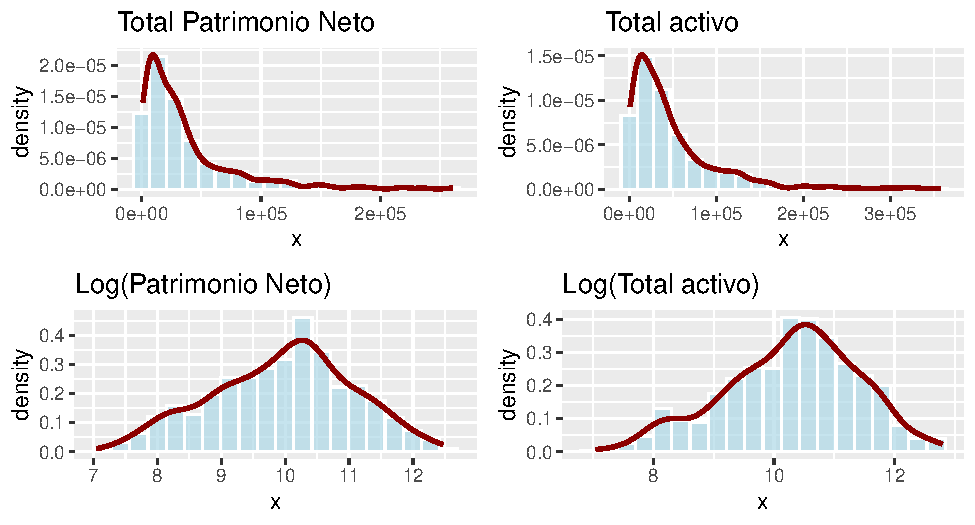
\includegraphics{CODIGO_PROYECTO_EM_files/figure-latex/unnamed-chunk-3-1.pdf}
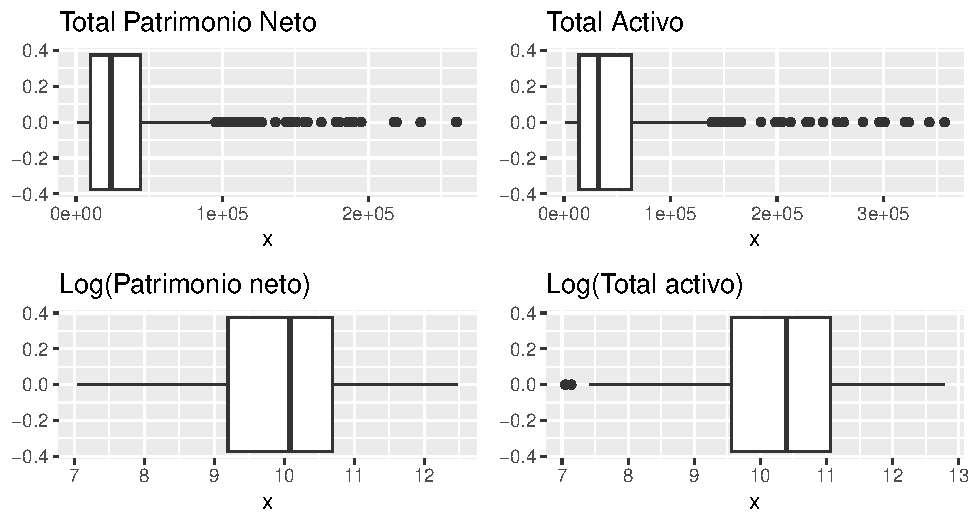
\includegraphics{CODIGO_PROYECTO_EM_files/figure-latex/unnamed-chunk-3-2.pdf}

Realizando esta transformación optenemos un \textbf{valor-p} de 0.4748
lo cual nos indica que no hay suficiente evidencia estadística para
rechazar la hipotesis nula , por tanto los datos provienen de una
distribución de mixturas normales.

Ya con esto se procede a ejecutar el algoritmo EM con el cual se
encuentra los parámetros de la distribución normal multivariante.Las
medias y matrices de varianza y covarianza de la subpoblación son las
siguientes

\begin{verbatim}
## number of iterations= 80
\end{verbatim}

\[\mu_1=[9.850069 ;10.47885]\] \[\mu_2=[10.032998; 10.12234]\]

\[
\sum_1 = \begin{bmatrix}
   1.025812 & 0.8741010 \\
   0.874101& 0.8984864 \\
\end{bmatrix}
\] \[
\sum_2 = \begin{bmatrix}
   1.352622 & 1.3783079 \\
   1.378308 & 1.4139173  \\
\end{bmatrix}
\]

y los pesos correspondientes son

\[\lambda_1=0.4434142 ; \lambda_2= 0.5565858\]

los resultados de este ajuste lo podemos ver a continuación

\begin{figure}[h]
  \centering
  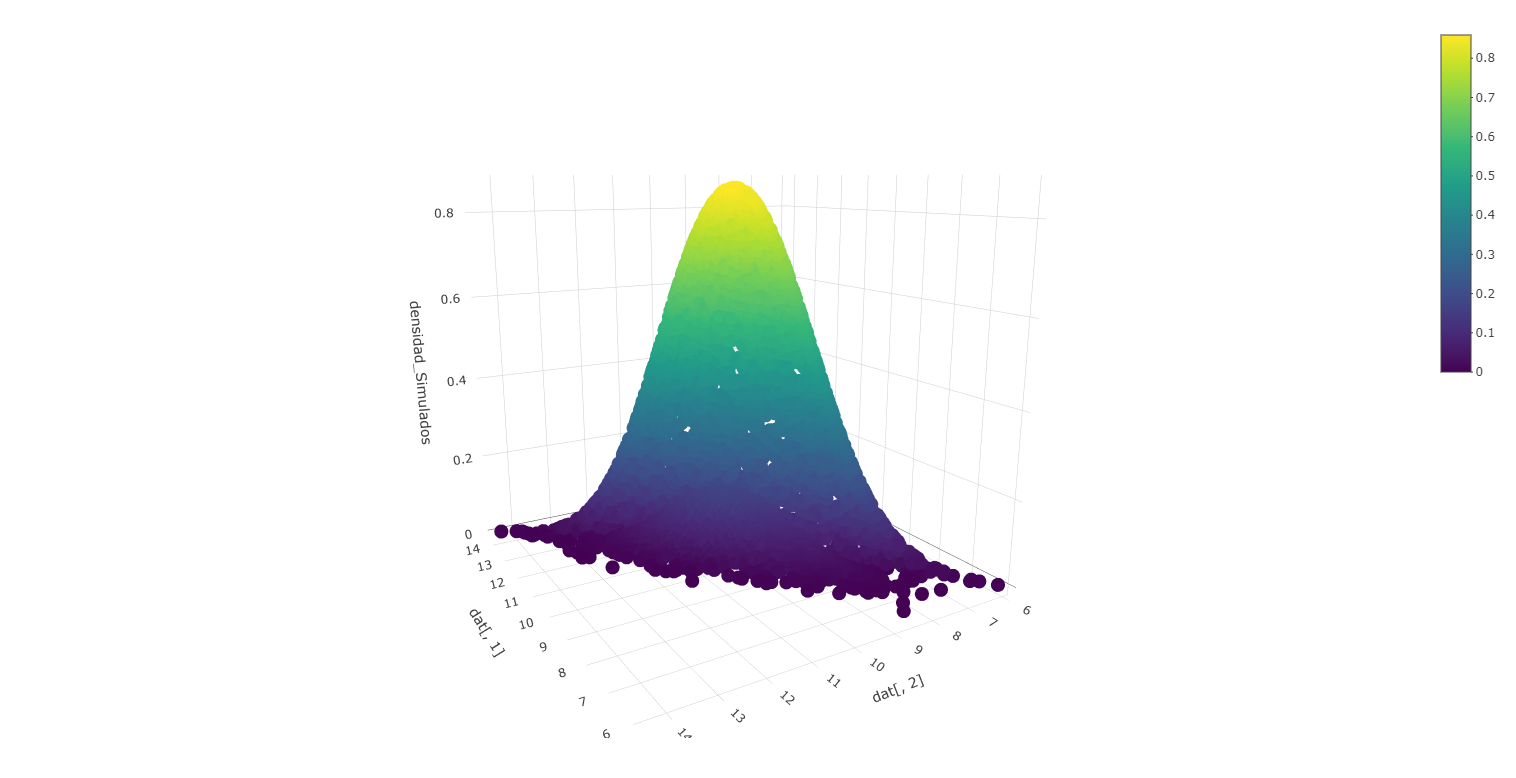
\includegraphics[width=0.8\linewidth]{simulados.png}
  \caption{Densidad Simulados}
  \label{fig:etiqueta}
\end{figure}

También podemos observar la gráfica correspondiente a los datos
originales transformados

\begin{figure}[h]
  \centering
  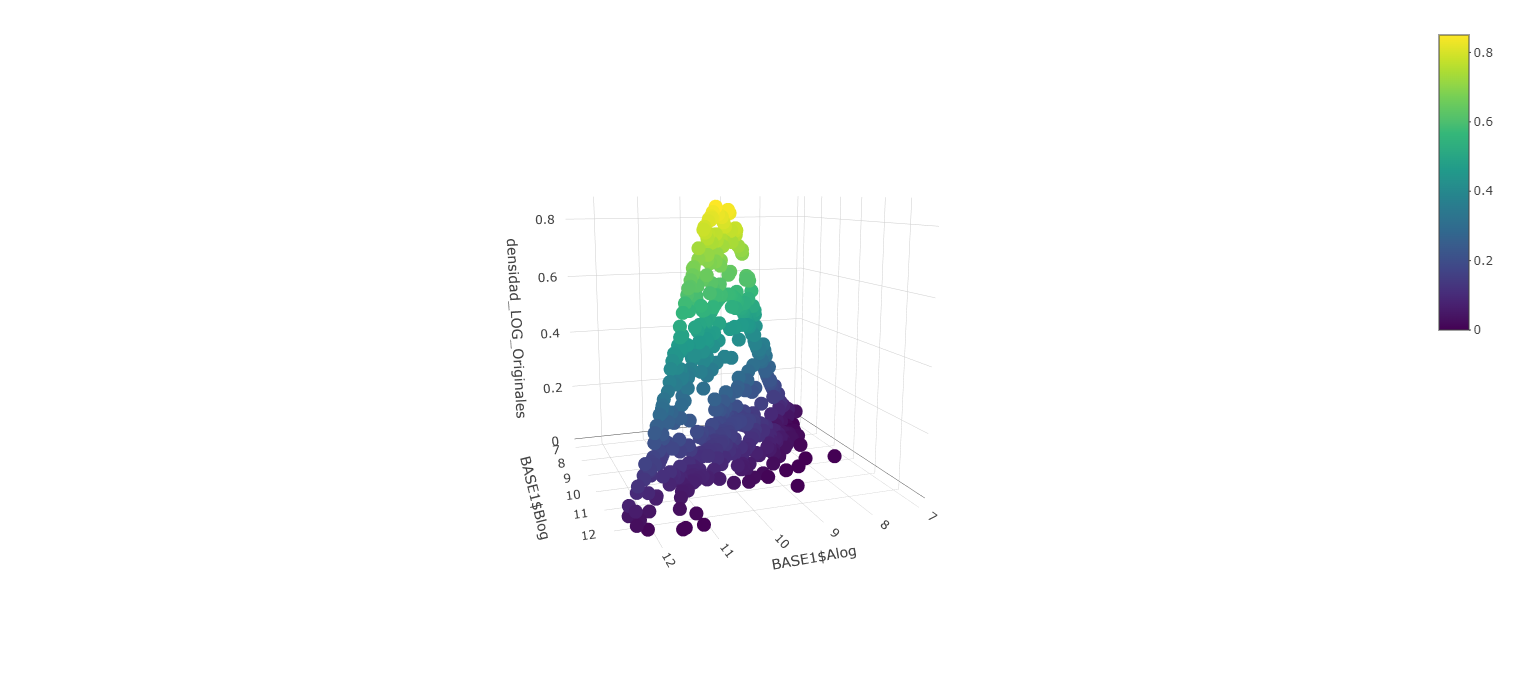
\includegraphics[width=0.8\linewidth]{originales.jpg}
  \caption{Densidad Originales transformados.}
  \label{fig:etiqueta}
\end{figure}

Del procedimiento anterior encontramos una distribución exacta (mixtura
de normales multivariante) que describe la distribución entre el
patrimonio neto transformado y los activos transformados . Ahora
mediante Montecarlo simulamos los datos requeridos para la construcción
del indicador de solvencia.

\includegraphics{CODIGO_PROYECTO_EM_files/figure-latex/unnamed-chunk-7-1.pdf}

Finalmente presentamos los resultados obtenidos de las simulaciones
realizadas

\begin{table}[!h]
    \centering
    \caption{\textbf{Estimaciones por Montecarlo y Bootstrap (Datos Transformados)}}
    \begin{tabular}{|l|l|l|l|l|l|}
    \hline
        Método/Medida & Media & Varianza & Sd & LINF & LimSUP \\ \hline
        Montecarlo & -0.3285 & 0.1554 & 0.3942 & -0.3396859 & -0.3179281 \\ \hline
        Bootstrap & -0.328538 & 0.235 & 0.221 & -0.3589944  & -0.2990529  \\ \hline
    \end{tabular}
\end{table}

Para el entendimiento de los resultados retransformamos los valores
estimados

\begin{table}[!h]
    \centering
    \caption{\textbf{Estimaciones por Montecarlo y Bootstrap (Datos Retransformados)}}
    \begin{tabular}{|l|l|l|l|l|l|}
    \hline
        Método & Media & Var & Sd & LINF & LSUP \\ \hline
        Montecarlo & 0.719 & 1.1681 & 1.483255 & 0.71326 & 0.72658 \\ \hline
        Bootstrap & 0.766 & 0.05147959 & 0.2268183 & 0.7491227 & 0.7837504 \\ \hline
    \end{tabular}
\end{table}

Podemos observar que el metodo por Montecarlo es más angosto que
bootstrap , pero en cambio este último presenta sesgos bastante pequeños
como se muestra a continuación.

\begin{table}[!h]
    \centering
    \caption{\textbf{Estimaciones por Montecarlo y Bootstrap (Datos Retransformados)}}
    \begin{tabular}{|l|l|l|l|}
    \hline
        Método & SESGO MEDIA & SESGO Varianza & SESGO Sd  \\ \hline
        Montecarlo & -0.0464 & 1.1166 & 0.1671 \\ \hline
        Bootstrap & -5.237828e-05 & 8.694168e-05  & 0.0002643589 \\ \hline
    \end{tabular}
\end{table}

Para la prueba de hipótesis el jefe según su experiencia segura que el
indice de solvencia en promedio es igual \(72\%\) . Por lo cual nuestra
prueba de hipótesis viene dada por

\[ H_0: \theta = 0.72 \] \[ H_a: \theta \neq 0.72 \]

Donde \$\theta \$ representa la media poblacional de nuestro estimador.

\begin{verbatim}
## 
## Proporción de rechazos al 1%= 0.008
\end{verbatim}

\begin{verbatim}
## 
## Proporción de rechazos al 5%= 0.049
\end{verbatim}

\begin{verbatim}
## 
## Proporción de rechazos al 10%= 0.1
\end{verbatim}

Esta salida proporciona información sobre la tasa de rechazo bajo
diferentes niveles de significancia, lo que es útil para evaluar el
poder estadístico del procedimiento.

\hypertarget{conslusiones-y-recomendaciones}{%
\section{Conslusiones y
recomendaciones}\label{conslusiones-y-recomendaciones}}

\hypertarget{anexos}{%
\section{Anexos}\label{anexos}}

\hypertarget{referencias}{%
\section{Referencias}\label{referencias}}

\emph{{[}1{]}} Guayasamín, P. (17 de septiembre de 2023). Simulación
Montecarlo y Bootstrap: Cooperativas deterioradas en el indicador de
liquidez diciembre 2022 - enero 2023.

\emph{{[}2{]}} Fernández-Casal, R., Cao, R., \& Costa, J. (2023).
Técnicas de Simulación y Remuestreo (github). Recuperado de
{[}\url{https://rubenfcasal.github.io/simbook/}{]}

\emph{{[}3{]}} Cao, R., \& Fernández-Casal, R. (2021). Técnicas de
Remuestreo (github). Recuperado de
{[}\url{https://rubenfcasal.github.io/book_remuestreo/}{]}

\end{document}
